\documentclass{article}
\usepackage{amsfonts}      
\usepackage{amsmath}
\usepackage{amssymb}
\usepackage{bm}
\usepackage{enumitem}
\usepackage{mdframed}
\usepackage{stackengine}
\usepackage{mathtools}
\usepackage{tabularx}
\usepackage{changepage}
\usepackage{dashrule}
\usepackage{nicefrac}
\usepackage{xfrac}
\usepackage{tikz}
\usepackage[margin=1mm, landscape, twocolumn]{geometry}
\newcommand{\R}{\mathbb{R}}
\newcommand{\Z}{\mathbb{Z}}
\newcommand{\E}{\mathbb{E}}
\newcommand{\I}{\mathbb{I}}
\newcommand{\T}{\bf{T}}
\newcommand{\QQ}{\bf{Q}}
\newcommand{\QT}{\bf{Q$^{\bf{T}}$}}
\newcommand{\QI}{\bf{Q$^{\bf{-1}}$}}
\newcommand{\A}{\bf{A}}
\newcommand{\AT}{\bf{A$^{\T}$}}
\newcommand{\X}{\bf{X}}
\newcommand{\Y}{\bf{Y}}
\newcommand{\x}{\bf{x}}
\newcommand{\w}{\bf{w}}
\newcommand{\y}{\bf{y}}
\renewcommand{\v}{\bf{v}}
\newcommand{\z}{\bf{z}}
\newcommand{\h}{\bf{h}}
\newcommand{\m}{\bf{m}}
\renewcommand{\a}{\bf{a}}
\newcommand{\g}{\bf{g}}
\renewcommand{\u}{\bf{u}}
\renewcommand{\b}{\bf{b}}
\newcommand{\B}{\bf{B}}
\newcommand{\U}{\bf{U}}
\newcommand{\V}{\bf{V}}
\newcommand{\W}{\bf{W}}

\newcommand{\ot}{\leftarrow}
\renewcommand{\bf}[1]{\textbf{{#1}}}
\renewcommand{\tt}[1]{\texttt{{#1}}}
\renewcommand{\it}[1]{\textit{{#1}}}
\newcommand{\ib}[1]{\textit{\textbf{{#1}}}}
\newcommand{\pd}[2]{\frac{\partial{#1}}{\partial{#2}}}
\newcommand{\grad}[2]{\nabla_{#1}{#2}}
\newcommand{\ul}[1]{\underline{{#1}}}
\newcommand{\relu}{\text{relu}}
\newcommand{\eps}{\varepsilon}
\renewcommand{\L}{\mathcal{L}}
\newcommand{\tbu}{\bf{\ul{}}}
\DeclareMathOperator*{\argmin}{arg\,min}
\DeclareMathOperator*{\var}{var}
\DeclareMathOperator*{\sm}{softmax}
\setlength\parindent{0pt}


\begin{document}
\begin{small}
\bf{Vector Derivatives}
\newline
Let $\x, \theta \in \R^n$
\newline
\bf{$\bm{\theta^T \x}$}: 
$
\grad{\x}{\theta^T \x} = \theta 
\mid 
\grad{\theta}{\theta^T \x} = \x
$
\newline
\bf{$\bm{\x^T \A \x}$}: 
$
\grad{\x}{\x^T \A \x} = (\A + \A^T) \x
\mid 
\grad{\A}{\x^T \A \x} = \x \x^T
\mid \A$ symmetric, then 
$\grad{\x}{\x^T \A \x} = 2\A \x$.
\hrule
\vspace{0.1em}

\bf{Matrix Derivatives}
\newline
Let $\z^T \in \R^m, \x \in \R^n, \A \in \R^{m \times n}$.
\newline
$
\R^{m \times n} \ni
\grad{\A}{\z^T \A \x} =
\begin{bmatrix}
    \pd{\x^T \A \x}{a_{ij}}
\end{bmatrix}
$ for $i = 1, \cdots, m$ and $j = 1, \cdots, n$
\vspace{0.1em}

\hrule
\vspace{0.1em}

\bf{General Formula:}
\newline
$y = \sum_{i = 0}^{n} a_i x^i$. Higher degrees always fit better, but this may lead to overfitting.
\vspace{0.1em}

\hrule
\vspace{0.1em}

\bf{Evaluating Generalization Error}
\newline
\bf{Training data} is what's used to learn $\theta$. \bf{Testing data} is data that the model has
never seen before. We typically want to do better on \ib{testing data}. \bf{Overfitting} is when the
model has \it{low} training error, but \it{high} testing error. More data helps mitigate
overfitting; $\it{more data} \implies \it{more complex models}$. \bf{Underfitting} is when a model 
has \it{high} training error and \it{high} testing error. \bf{Hyperparameters} are parameters chosen
before we start training. \bf{Validation} data is data used to optimize the \it{hyperparameters}.
All of these datasets are disjoint.
\hrule
\vspace{0.1em}

\bf{$\bm{k}$-fold Cross Validation}
\newline
If our \bf{training data} has $N$ examples, pick any $k \in \Z^{> 0}$. Define each fold to have $N/k$
examples. Then, $k - 1$ folds are used to train the model and learn $\theta$. The $k^{th}$ fold is 
\bf{validation data} used to evaluate the model. We can repeatedly train the model by changing which
folds are for \bf{training} and \bf{validation}. Then 
$k - 1 \ \it{folds} \to \theta, k^{th} \ \it{fold} \to \L$.
\hrule
\vspace{0.1em}

\bf{Data Driven Approach}
\newline
We \it{train} on data to get model parameters $\theta$. In deep NN's, this results in learning
\it{features} that are optimized for image classification. Here, 
$
\it{features}\footnote
{$\hat{\x}$ is the vectorzed version of $1, \cdots x^n$ in $\y := \sum_{i = 0}^{n} a_i x^i$} 
:= \hat{\x} =
\begin{bmatrix}
    x^n & \cdots & 1
\end{bmatrix}^T
$
are inferred by the training data. We then \it{test} our model to classify new images.
\hrule
\vspace{0.1em}

\bf{K-Nearest Neighbors (KNN)}
\newline
Find the $k$-closest points to $\x^{\it{new}}$ in the training set, according to an appropriate 
metric (e.g. $L_2$). Then the majority vote is the class $\x^{\it{new}}$ is assigned to.
\bf{Formally:} Define the distance metric $d(\x^{\it{new}}, \x^{(i)})$. Choose $k \in \Z^{> 0}$.
Take $d(\x^{\it{new}}, \x^{(i)})$ for $i = 1, \ldots, m$ and find the $k$ nearest neighbors 
$\{c_1, \cdots c_k\}$. Take the plurality vote (randomizing ties) to classify $\x^{\it{new}}$. Here,
the hyperparameters are $\{k, d(\cdot)\}$
\newline
\bf{Issues for Image Classification}
\newline
\bf{(i)} \it{pixel differences $\neq$ semantic differences}. If we transform the image, per pixel, 
the image is different, but the image is the same.
\bf{(ii)} The curse of dimensionality: As $n \to \infty$, the notion of ``distance'' becomes harder
to define and volume increases exponentially.
\hrule
\vspace{0.1em}

\bf{Softmax Classifier}
\newline
We want to ``score'' an image against each class and pick the class with the highest score.
\newline
\bf{Example:} Let 
$
\W := 
\begin{bmatrix}
    \w_1^T & \cdots & \w_c^T
\end{bmatrix}^T
\in \R^{10 \times 3072},
c = 10, \x \in \R^{3072}, \y, \b \in \R^{10}
$. Then $\y$ is the vector containing the score for class $i$. The chosen class is $i$ s.t. 
$y^{(i)} := \max\{\y\}$, where $\y$ is
\vspace{-1em}
\[
    \y := 
    \begin{bmatrix}
        \text{--- } \w_1^T \text{ ---} \\
        \vdots \\
        \text{--- } \w_{10}^T \text{ ---}
    \end{bmatrix}
    \begin{bmatrix}
        \\
        \x \\
        \\
    \end{bmatrix}
    +
    \begin{bmatrix}
        \\
        \b \\
        \\
    \end{bmatrix}
    =
    \begin{bmatrix}
        \w_1^T \x + b_1 \\
        \vdots \\
        \w_{10}^T \x + b_1 \\
    \end{bmatrix}
    \vspace{-1em}
\]
\bf{What a Linear Classifier Does}
\newline
Let $\x \in \R^2, y_1 = \w_1^T \x$. Then 
$
\ul{y_1}
= \|\w_1\| \|\x\| \cos(\theta) 
= \ul{\|\x\| \cos(\theta)}$ when $\|\w_1\| = 1$.
\newline
\bf{INSERT THE PICTURE}
\newline
Linear classifiers fail for things like \bf{xor}.
\hrule
\vspace{0.1em}

\bf{Chain Rule for Probability}
\newline
$p(a, b) = p(a)p(b \mid a) = p(b)p(a \mid b)$
\newline
$p(a, b, c) 
= p(c)p(a \mid c)p(b \mid a, c)
= p(a)p(b \mid a)p(c \mid a, b)
= p(a, c)p(b \mid a, c)
$
\newline
$p(b, c \mid d, e) = \frac{p(b, c, d, e)}{p(d)p(e \mid d)}$
\newline
$p(d \mid e) p (b, c \mid d, e) = \frac{p(a, b, c, d, e)}{p(a \mid b, c, d, e)}$

\newpage
\bf{Softmax}
\newline
$\sm_{i} (\x) := \frac{e^{\w_i^T \x + b_i}}{\sum_{j = 1}^{c} e^{\w_j^T + \x + b_j}}$. If we define
$a_i (\x) := \w_i^T \x + b_i$, we get $\sm_i (\x) = \frac{e^{a_i (\x)}}{\sum_{j = 1}^{c} e^{a_i (\x)}}$.
$a_i (\x)$ is the score of the image $\x$ being in the $i^{th}$ class and $\sm_{i} (\x)$ is the
probability of $\x$ being in the $i^{th}$ class.
\vspace{-0.5em}
\newline
\bf{Notation:} Define 
$
\widetilde{\w}_i^T := 
\begin{bmatrix}
    \w_i^T & b_i
\end{bmatrix}
,
\widetilde{\x} := 
\begin{bmatrix}
    \x \\ 1
\end{bmatrix}
$. Then $a_i (\widetilde{\x}) = \widetilde{w}_i^T \widetilde{\x}$, 
$\sm_i (\widetilde{\x}) = \frac{e^{a_i (\widetilde{\x})}}{\sum_{j = 1}^{c} e^{a_i (\widetilde{\x})}}$,
so the probability that $\x^{(j)}$ belongs to class $i$ is given by:
$\Pr(y^{(j)} = i \mid \x^{(j)}, \theta) = \sm_{i} (\x^{(j)})$
\hrule
\vspace{0.1em}

\bf{Cross Entropy Loss}
\newline
$
\L 
:= \argmin\limits_{\theta} 
\frac{1}{m} \sum\limits_{i = 1}^{m} 
\left( \log \left[ \sum\limits_{j = 1}^{c} e^{a_j (\x^{(i)})} \right] - a_{y^{(i)}} x^{(i)} \right)
$
\newline
For binary classification problems:
$\L := - \sum\limits_{i = 1}^{m} (y_i \log[\sigma(z)] + (1 - y_i)\log[1 - \sigma(z)])$.
Then the gradient is
$\grad{\sigma(z)}{\L} = \frac{y_i}{\sigma(z)} - \frac{1 - y_i}{1 - \sigma(z)}$
The parameters for $\L$ are $\theta = \{\W, \b\}$ where $\W \in \R^{c \times n}, \b \in \R^c$.
\hrule
\vspace{0.1em}
\bf{Gradient Descent}
\newline
Recall that for $\eps > 0$ sufficiently small, $f(x + e) \approx f(x) + \eps f'(x)$. Let
$\L := f, x = \theta$. Then, for $n$-dimensional loss landscapes, we have $n$ search
dimensions to make $\L(\theta) \to 0$. As $n \to \infty$, the local minima $\to$ global
minimum. So 
$
\L(\theta + \Delta \theta) 
\approx 
\L(\theta) + \Delta \theta^T \grad{\theta}{\L(\theta)}
$. To minimize $\L$, we need to find 
$
\min\limits_{\u, \|\u\| = 1} \u^T \grad{\theta}{\L(\theta)}
=
\min\limits_{\u, \|\u\| = 1} \|\u\| \|\grad{\theta}{\L(\theta)}\| \cos(\theta)
=
\min\limits_{\u} \|\grad{\theta}{\L(\theta)}\| \cos(\theta)
$ which is minimized when $\cos(\theta) = -1$, so $\u := -\grad{\theta}{\L(\theta)}$. Then we
repeatedly calculate $\theta \ot \theta - \eps \grad{\theta}{\L(\theta)}$. 
\newline
\bf{Why Not Numerical?} There are too many parameters. Takes too much time.
\newline
\bf{Intuition:}
The gradient w.r.t. the parameters is a function of the training data. We can think of each point as
a noisy estimate of the gradient at that point.
\hrule
\vspace{0.1em}

\bf{Batch v. Minibatch}
Given $m$ examples:
\newline
\bf{Batch:} uses all $m$ examples in the training data to calculate the gradient.
\bf{Minibatch:} approximates the gradient by using $k$ examples for computation, where $1 < k < m$.
\bf{Stochastic:} approximates the gradient over one example.
We typically use minibatching for neural networks. Minibatch \it{may} be referred to SGD.
\hrule
\vspace{0.1em}
\bf{Nomenclature:} The \bf{input layer} is the first layer of the NN, typically $\x$.
The \bf{output layer} is the last layer of the NN, typically $\z$. The \bf{hidden layers} are the
intermediate layers of the NN, typically $\h_i$. For a NN with $N$ layers, we \ib{do not} count the
input layer as part of $N$. Note that $\z$ are the scores that go a softmax classifier, sometimes
called ``logits''.
\newline
\bf{Example}
\newline
Let $\h_1 = \W_1 \x + \b_1$, $\h_i = \W_i \h_{i - 1} + \b_1$ for $i = 2, \cdots, N - 1$, 
$\z = \W_N \h_{N - 1} + \b_N$. Then $\z = \widetilde{\W} \x + \widetilde{\b}$ where 
$\widetilde{\W} = \W_N \cdots \W_1$ and 
$\widetilde{\b} = \b_N + \sum_{i = 2}^{N - 1} \W_i \b_{i - 1}$.
\newline
\bf{Linear $\bm{f}$:} $f(x) = ax + b$ can be useful if $\dim(\h) \ll \dim(\x)$. This corresponds to
finding a low-rank representation of the inputs (e.g. autoencoder).
\newline
$f$ is the \bf{activation function} and is typically \ib{not} applied to $\z$.
\newline
\bf{Hidden Layers as Learned Features:} Nonlinear $f(\h_i)$ finds features of the data. If $\sm(\z)$
is good, then $\h_i$ is linearly separable.
\newline
\bf{Learnable Parameters:} 
$
\left(
    |\x| \cdot |\h_1| 
    + 
    \left( \sum_{i = 1}^{N - 2} |\h_i| \cdot |\h_{i + 1}| \right) 
    + 
    \h_{N - 1} \cdot |\z|
\right)
+
\left(
    |\z| + \sum_{i = 1}^{N - 1} |\h_i|
\right)
$.
\vspace{0.1em}

\hrule
\vspace{0.1em}

\bf{Activation Functions}
\newline
\ul{\bf{Sigmoid:}} $\sigma (x) = \frac{1}{1 + e^{-x}}$. $\grad{x}{\sigma} = \sigma(x)(1 - \sigma(x))$.
\newline
\bf{Vanishing Gradient Problem:} We want $\grad{\w}{\L}$ to be large since 
$\w \ot \w - \eps \grad{\w}{\L}$. Then we have $f(\w_1^T \x + \b) =: \sigma(\w)$, so 
$\pd{\L}{\w} = \pd{\sigma}{\w} \cdot \pd{\L}{\sigma}$. For extreme inputs, there is no learning 
since $\pd{\L}{\w} \approx 0$, so $\w \ot \w + 0$ (saturation). $\sigma$ can have zig-zagging 
gradients since $\sigma$ is always nonnegative.
\newline
\bf{Output Activations:} $\hat{y}^{(i)} = \sm_i(\z)$ is the generalization of $\sigma$ to multiple
classes.
\newline
\ul{\bf{ReLu:}} $\relu(x) = \max\{0, x\}$. 
$
\grad{x}{\relu} =
\begin{cases}
    1 & x > 0 \\
    0 & \it{else}
\end{cases}
$. ReLu is widely used in practice. It can still have zig-zagging gradients but there is no
saturation.
\newline
\ul{\bf{$\bm{\tanh}$:}} $\tanh(x) = 2\sigma(2x) - 1$. 
$\grad{x}{\tanh} = 1 - \tanh^2(x)$ It is zero-centered so there is no vanishing
gradient problem, but there's still saturation for extreme inputs.

\newpage
\bf{Deep Learning Architecture:}
\it{Input $\to$ Hidden $\to$ Output} $\to \sm \to \L$. 
\bf{Loss function:} $\sm_i (\z)$.
\bf{Learning role:} $\theta \ot \theta - \eps \grad{\theta}{\L}$.
\hrule
\vspace{0.1em}

\bf{Nomenclature}
\newline
\bf{Forward pass} is $\x \to \cdots \to \z \to \L$. \bf{Backpropagation} is
$\pd{\L}{\z} \to \cdots \to \pd{\L}{\theta_1}$. Backpropagation operationalizes the gradient. It is
computationally efficient since we cache values during forward pass to use during the backward pass.
In general, we have
\vspace{-1em}
\begin{center}
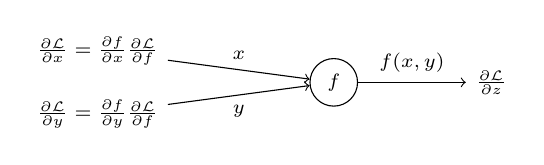
\begin{tikzpicture}[font=\scriptsize]
    \node (x) at (0, 0.4) {$\pd{\L}{x} = \pd{f}{x} \pd{\L}{f}$};
    \node (y) at (0, -0.4) {$\pd{\L}{y} = \pd{f}{y} \pd{\L}{f}$};
    \node (f) [draw, circle] at (3, 0) {\(f\)};
    \node (output) at (5, 0) {$\pd{\L}{z}$};

    \draw[->] (x) -- (f) node[midway, above] {$x$};
    \draw[->] (y) -- (f) node[midway, below] {$y$};
    \draw[->] (f) -- (output) node[midway, above] {$f(x, y)$};
\end{tikzpicture}
\vspace{-1em}
\end{center}
where $\pd{f}{x}, \pd{f}{y}$ are local gradients and $\pd{\L}{f}$ is the upstream gradient.
\hrule
\vspace{0.1em}
\bf{Gates}
\newline
\ul{\bf{Addition:}} Distribute the upstream gradient $\pd{\L}{f}$.
\vspace{-1em}
\begin{center}
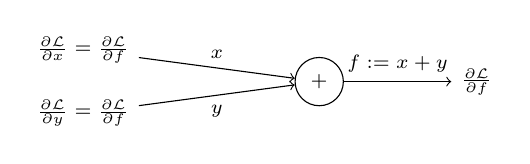
\begin{tikzpicture}[font=\scriptsize]
    \node (x) at (0, 0.4) {$\pd{\L}{x} = \pd{\L}{f}$};
    \node (y) at (0, -0.4) {$\pd{\L}{y} = \pd{\L}{f}$};
    \node (f) [draw, circle] at (3, 0) {$+$};
    \node (output) at (5, 0) {$\pd{\L}{f}$};

    \draw[->] (x) -- (f) node[midway, above] {$x$};
    \draw[->] (y) -- (f) node[midway, below] {$y$};
    \draw[->] (f) -- (output) node[midway, above] {$f := x + y$};
\end{tikzpicture}
\vspace{-1em}
\end{center}
\ul{\bf{Multiplication (Scalar):}} Switch $x, y$ and multiply by the upstream gradient $\pd{\L}{f}$.
\vspace{-1em}
\begin{center}
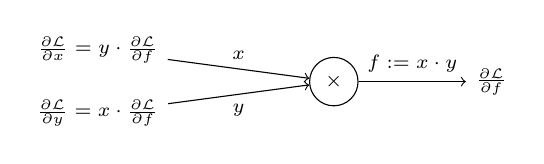
\begin{tikzpicture}[font=\scriptsize]
    \node (x) at (0, 0.4) {$\pd{\L}{x} = y \cdot \pd{\L}{f}$};
    \node (y) at (0, -0.4) {$\pd{\L}{y} = x \cdot \pd{\L}{f}$};
    \node (f) [draw, circle] at (3, 0) {$\times$};
    \node (output) at (5, 0) {$\pd{\L}{f}$};

    \draw[->] (x) -- (f) node[midway, above] {$x$};
    \draw[->] (y) -- (f) node[midway, below] {$y$};
    \draw[->] (f) -- (output) node[midway, above] {$f := x \cdot y$};
\end{tikzpicture}
\vspace{-1em}
\end{center}
\ul{\bf{Multiplication ($\bm{n}$-Dimensional Vector/Tensor):}} Fancy tensor derivative shortcut.
\vspace{-1em}
\begin{center}
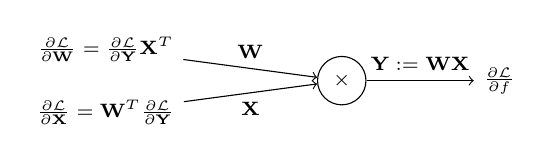
\begin{tikzpicture}[font=\scriptsize]
    \node (w) at (0, 0.4) {$\pd{\L}{\W} = \pd{\L}{\Y} \X^T$};
    \node (x) at (0, -0.4) {$\pd{\L}{\X} = \W^T \pd{\L}{\Y}$};
    \node (f) [draw, circle] at (3, 0) {$\times$};
    \node (output) at (5, 0) {$\pd{\L}{f}$};

    \draw[->] (w) -- (f) node[midway, above] {$\W$};
    \draw[->] (x) -- (f) node[midway, below] {$\X$};
    \draw[->] (f) -- (output) node[midway, above] {$\Y := \W \X$};
\end{tikzpicture}
\vspace{-1em}
\end{center}
\ul{\bf{Max:}} Route the upstream gradient $\pd{\L}{f}$.
\vspace{-1em}
\begin{center}
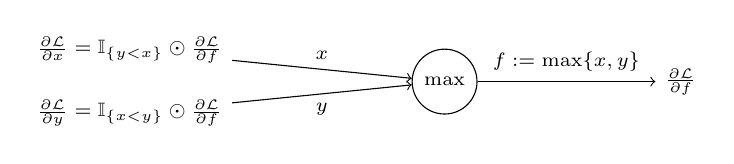
\begin{tikzpicture}[font=\scriptsize]
    \node (x) at (0, 0.4) {$\pd{\L}{x} = \I_{\{y < x\}} \odot \pd{\L}{f}$};
    \node (y) at (0, -0.4) {$\pd{\L}{y} = \I_{\{x < y\}} \odot \pd{\L}{f}$};
    \node (f) [draw, circle] at (4, 0) {$\max$};
    \node (output) at (7, 0) {$\pd{\L}{f}$};

    \draw[->] (x) -- (f) node[midway, above] {$x$};
    \draw[->] (y) -- (f) node[midway, below] {$y$};
    \draw[->] (f) -- (output) node[midway, above] {$f := \max\{x, y\}$};
\end{tikzpicture}
\vspace{-1em}
\end{center}
\ul{\bf{ReLu:}} Hadamard product the upstream gradient $\pd{\L}{f}$.
\vspace{-1em}
\begin{center}
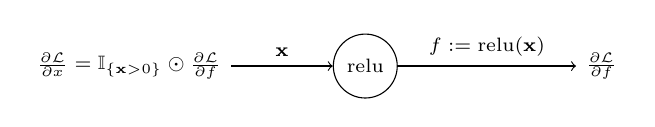
\begin{tikzpicture}[font=\scriptsize]
    \node (x) at (0, 0) {$\pd{\L}{x} = \I_{\{\x > 0\}} \odot \pd{\L}{f}$};
    \node (f) [draw, circle] at (3, 0) {$\relu$};
    \node (output) at (6, 0) {$\pd{\L}{f}$};

    \draw[->] (x) -- (f) node[midway, above] {$\x$};
    \draw[->] (f) -- (output) node[midway, above] {$f := \relu(\x)$};
\end{tikzpicture}
\vspace{-1em}
\end{center}
\ul{\bf{$\bm{f^{-1}}$:}} Derivative of $\nicefrac{1}{x}$ multiplied by the upstream gradient $\pd{\L}{f}$.
\vspace{-1em}
\begin{center}
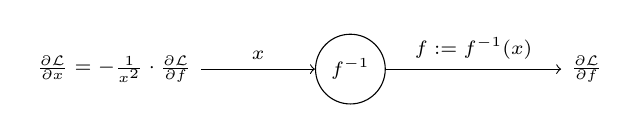
\begin{tikzpicture}[font=\scriptsize]
    \node (x) at (0, 0) {$\pd{\L}{x} = -\frac{1}{x^2} \cdot \pd{\L}{f}$};
    \node (f) [draw, circle] at (3, 0) {$f^{-1}$};
    \node (output) at (6, 0) {$\pd{\L}{f}$};

    \draw[->] (x) -- (f) node[midway, above] {$x$};
    \draw[->] (f) -- (output) node[midway, above] {$f := f^{-1}(x)$};
\end{tikzpicture}
\vspace{-1em}
\end{center}
\ul{\bf{$\bm{e^x}$:}} Derivative of $e^x$ multiplied by the upstream gradient $\pd{\L}{f}$.
\vspace{-1em}
\begin{center}
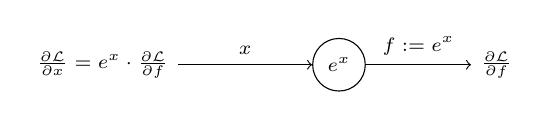
\begin{tikzpicture}[font=\scriptsize]
    \node (x) at (0, 0) {$\pd{\L}{x} = e^x \cdot \pd{\L}{f}$};
    \node (f) [draw, circle] at (3, 0) {$e^x$};
    \node (output) at (5, 0) {$\pd{\L}{f}$};

    \draw[->] (x) -- (f) node[midway, above] {$x$};
    \draw[->] (f) -- (output) node[midway, above] {$f := e^x$};
\end{tikzpicture}
\vspace{-1em}
\end{center}
\ul{\bf{$\bm{x^n}$:}} Derivative of $x^n$ multiplied by the upstream gradient $\pd{\L}{f}$.
\vspace{-1em}
\begin{center}
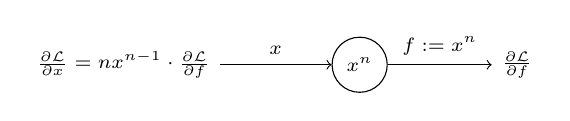
\begin{tikzpicture}[font=\scriptsize]
    \node (x) at (0, 0) {$\pd{\L}{x} = nx^{n - 1} \cdot \pd{\L}{f}$};
    \node (f) [draw, circle] at (3, 0) {$x^n$};
    \node (output) at (5, 0) {$\pd{\L}{f}$};

    \draw[->] (x) -- (f) node[midway, above] {$x$};
    \draw[->] (f) -- (output) node[midway, above] {$f := x^n$};
\end{tikzpicture}
\vspace{-1em}
\end{center}
\ul{\bf{$\bm{\sqrt{x}}$:}} Derivative of $\sqrt{x}$ multiplied by the upstream gradient $\pd{\L}{f}$.
\vspace{-1em}
\begin{center}
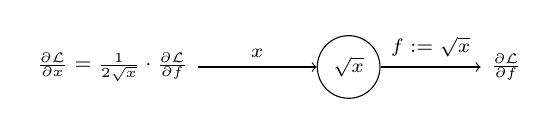
\begin{tikzpicture}[font=\scriptsize]
    \node (x) at (0, 0) {$\pd{\L}{x} = \frac{1}{2\sqrt{x}} \cdot \pd{\L}{f}$};
    \node (f) [draw, circle] at (3, 0) {$\sqrt{x}$};
    \node (output) at (5, 0) {$\pd{\L}{f}$};

    \draw[->] (x) -- (f) node[midway, above] {$x$};
    \draw[->] (f) -- (output) node[midway, above] {$f := \sqrt{x}$};
\end{tikzpicture}
\vspace{-1em}
\end{center}
\ul{\bf{Law of Total Derivatives}}
\vspace{-1em}
\begin{center}
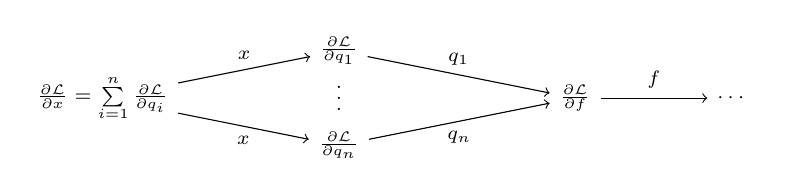
\begin{tikzpicture}[font=\scriptsize]
    \node (x) at (0, 0) {$\pd{\L}{x} = \sum\limits_{i = 1}^{n} \pd{\L}{q_i}$};
    \node (dots) at (3, 0.1) {$\vdots$};
    \node (q1) at (3, 0.6) {$\pd{\L}{q_1}$};
    \node (qn) at (3, -0.6) {$\pd{\L}{q_n}$};
    \node (f) at (6, 0) {$\pd{\L}{f}$};
    \node (output) at (8, 0) {$\cdots$};

    \draw[->] (x) -- (q1) node[midway, above] {$x$};
    \draw[->] (x) -- (qn) node[midway, below] {$x$};
    \draw[->] (q1) -- (f) node[midway, above] {$q_1$};
    \draw[->] (qn) -- (f) node[midway, below] {$q_n$};
    \draw[->] (f) -- (output) node[midway, above] {$f$};
\end{tikzpicture}
\vspace{-1em}
\end{center}
\bf{Multivariate Chain Rule:} 
$\grad{\x}{\z} = \grad{\x}{\y} \cdot \grad{\y}{\z} 
= \pd{\y}{\x} \cdot \pd{\z}{\y} = \pd{\z}{\x}$

\newpage
\bf{Regularization}
\newline
\bf{Initialization:} Weight initialization can heavily impact the performance of a NN. \bf{Small} 
random weight initialiations cause all activations to go to 0 since $\pd{\L}{\theta_i} \to 0$.
\bf{Large} random weight initializations cause all activations to go to $\infty$ since
$\pd{\L}{\theta_i} \to \infty$.
\newline
\bf{Xavier Initialization}
\newline
Try to keep the variences between layers equal: 
$\var(h_i) \approx \var(h_j) \implies \var(\grad{h_i}{L}) \approx \var(\grad{h_j}{\L})$.
\newline
\bf{Derivation:} Suppose all units are linear; i.e. 
$h_i := \sum_{j = 1}^{n_{\it{in}}} w_{ij} h_{i - 1, j}$ and suppose $w_{ij}, h_{i - 1, j}$ are
independent. Then
$\ul{\var(wh)} = \E^2(w) \var(h) + \E^2(h) \var(w) + \var(w) \var(h) = \ul{\var(w) \var(h)}$ if 
$\E(w) = \E(h) = 0$. Then 
$\ul{\var(h_i)} = \var\left( \sum_{j = 1}^{n_{\it{in}}} w_{ij} h_{i - 1, j} \right)
= \ul{\var(h_{i - 1}) \cdot \sum_{j = 1}^{n_{\it{in}}} \var(w_{ij})}
\implies 
\sum_{j = 1}^{n_{\it{in}}} \var(w_{ij}) = 1$ to get $\var(h_i) = \var(h_{i - 1})$.
Assuming the weights have the same statistics, 
$n_{\it{in}} \cdot \var(w) = 1 \implies \var(w) = \frac{1}{n_{\it{in}}}$. So 
$\var(w_{ij}) = \frac{1}{n_{\it{in}}}$.
Similarly for backprop, 
$\var(w_{ij}) = \frac{1}{n_{\it{out}}}$, so 
$\var(w_{ij}) = \frac{2}{n_{\it{in}} + n_{\it{out}}} = \frac{1}{n_{\it{avg}}}$.
\vspace{0.1em}

\hrule
\vspace{0.1em}

\bf{Batch Normalization}
\newline
We want to avoid saturation and high variance in activiations. The issue is that the changes we make
at each gradient step affects the other layers. For example, $\W_3 \ot \W_3 - \eps
\frac{\partial \L}{\partial \W_3}$ changes $\h_3$ based on $\h_2$, but $\h_2$ may also change
due to $\W_2 \ot \W_2 - \eps \frac{\partial \L}{\partial \W_3}$. By induction, we see that the issue 
propagates. The idea of \bf{batch normalization} is to make the output of each layer have \it{unit
statistics}: $\h_i = \relu(x_i), \E(x_i) = 0, \var(x_i) = 1$.
\newline
\bf{Vanilla:}
\it{affine} $\to \relu \to$ \it{affine} $\to \relu$
\newline
\bf{Batch Normalization:}
\it{affine} $\to$ batch-norm $\to \relu \to$ \it{affine} $\to$ batch-norm $\to \relu$
\newline
\bf{Other Bullshit (HW):}
\it{affine} $\to \relu \to$ batch-norm $\to$ \it{affine} $\to \relu \to$ batch-norm
\newline
Batch norm meets the \ib{Xavier Initialization} criteria ($\var(h_i) \approx \var(h_j)$), so you
don't need to use Xavier but it's still good to.
\vspace{0.1em}

\hrule
\vspace{0.1em}

\bf{Normalizing Unit Activations}
\newline
Given a batch of $m$ samples, the \bf{normalized value} of the $i^{th}$ activation is defined as 
\vspace{-0.5em} 
$\hat{x}_i := \frac{x_i - \mu_i}{\sqrt{\sigma_i^2 + \eps}}$ where 
$\mu_i = \frac{1}{m} \sum_{j = 1}^{m} x_i^{(j)}$ is the \bf{mean} and 
$\sigma_i^2 = \frac{1}{m} \sum_{j = 1}^{m} \left( x_i^{(j)} - \mu_i \right)^2$ is the \bf{variance} 
of the activations across the batch. We then \ib{scale} and \ib{shift} the normalized activations
using learned parameters $\gamma$ and $\beta$ respectively, to get the \bf{output}
$y_i = \gamma_i \hat{x}_i + \beta_i$.
\newline
\bf{Training:} During \it{training}, we normalize the output of a layer for each minibatch. We also
compute a running mean and varience of the past $k$ minibatches for $1 \leq k \leq N$. We learn 
$\gamma$ and $\beta$ via \ib{backpropagation} in addition to $\theta$.
\newline
\bf{Testing:} During \it{testing}, we use the running mean and variance computed during
\it{training} to normalize each layer. Additionally, we use the $\gamma$ and $\beta$ that were
learned during \it{training}.
\vspace{0.1em}

\hrule
\vspace{0.1em}

\bf{Regularization} is any modification that improves testing/validation error but doesn't decrease
training error. (e.g. Stopping early)

\bf{Parameter Norm Penalty}
\newline
The \bf{parameter norm penalty is} denoted as $\Omega(\theta)$ where $\Omega$ is a hyperparameter
like $\L$. The cost function then becomes 
$\L := \L(\theta \mid \X, \y) + \alpha \Omega(\theta)$ where $\alpha \geq 0$ weights
$\Omega(\theta)$.
\newline
\bf{$\bm{L_2}$ Regularization}
\newline
$\Omega(\theta) = \frac{1}{2} \w^T \w = \frac{1}{2} \|\w\|^2$ promotes models with parameters close
to 0. That is, we want the norms to be small. $\pd{\Omega}{\W} = \W$, so our gradient step looks
like 
$
\widetilde{\L}(\theta \mid \X, \y) 
= \L(\theta \mid \X, \y) + \frac{\alpha}{2} \w^T \w
\to \grad{\w}{\widetilde{\L}} = \grad{\w}{\widetilde{\L}} + \alpha \w
\implies \w \ot \w - \eps \grad{\w}{\widetilde{\L}} 
\iff \w \ot (1 - \eps \alpha) \w - \eps \grad{\w}{\L}
$. We want small weights because large weights are more sensitive to variable inputs which leads to
overfitting.
\newline
\bf{Extensions:} If we know $\w$ is close to some $\b$, set $\Omega(\theta) = \|\w - \b\|_2^2$. More
generally, if we need two weights $\w^{(i)}, \w^{(j)}$ to be close, set 
$\Omega(\theta) = \|\w^{(i)} - \w^{(j)}\|_2^2$
\newline
\bf{$\bm{L_1}$ Regularization}
\newline
$\Omega(\theta) = \|\w\|_1 = \sum_{i} |w_i|$. This may be used for feature selection by pruning
weights that are 0.
\newline
\bf{Sparse Representation}
\newline
$\Omega(\h_i) = \|\h_i^{(i)}\|$.

\newpage
\bf{Dataset Augmentation}
\newline
We can \bf{augment} (e.g. crop, reflection, gaussian blur, etc.) the original image(s) to increase 
the size of the training data and also make the NN more robust to augmented data. 
\newline
\bf{Label Smoothing:} Adding noise helps to reduce error. We go from a \it{one hot} representation to 
\bf{label smoothing}:
$\L^{(i)} = \sum_{c = 1}^{C} -y_c \log(p_c) 
\to \L^{(i)} = \sum_{c = 1}^{C} -y_c(1 - \alpha) + \frac{\alpha}{C - 1}$ where $\alpha$ is a
hyperparameter.
\hrule
\vspace{0.1em}

\bf{Transfer Learning}
\newline
Training a NN in one context and using them in another with minimal additional training.
\newline
\bf{Ensemble Methods}
\newline
Training multiple different models and averaging their results at test time.
\newline
\bf{Intuition:} Independent models make independent errors.
\newline
\bf{Why this works:}
For one model, $\E(\eps^2)$. Then, 
$\E(\eps_i \eps_j) = \E(\eps_i) \E(\eps_j)$ if $\eps_i \perp \!\!\! \perp \eps_j$. Then
$
\E\left[ \left( \frac{1}{k} \sum_{i = 1}^{k} \eps_i \right)^2 \right]
=
\left( \frac{1}{k} \sum_{i = 1}^{k} \E(\eps_i) \right)^2
=
\frac{1}{k} \E(\eps_i)^2
$.
If $\eps_i \not \! \perp \!\!\! \perp \eps_j$, then 
$\frac{1}{k} \E(\eps_i)^2 + \frac{k - 1}{k} \E(\eps_i \eps_j)^2$
If the models are perfectly correlated, we get $\E(\eps_i)^2$. So we are bounded below and above.
\vspace{0.1em}

\hrule
\vspace{0.1em}
\bf{Bagging (Bootstrap Aggregating)}
\newline
Constuct $k$ datasets by drawing $N$ examples \it{with} replacement for each $i = 1, \cdots, k$.
Train $k$ models and \ib{ensemble}.
\vspace{0.1em}

\hrule
\vspace{0.1em}
\bf{Dropout}
Set a hyperparameter $p$ to be the probability of keeping a neuron in a layer. On any \it{training} 
iteration, draw a sample \it{binary mask} $\m$. Then $\h \odot \m$ ``drops'' $h_j \in \h$ where $m_j = 0$.
At \it{test} time, we do $\h_{\it{out}} = \relu\left( p \cdot \sum_{i = 1}^{n} w_i h_i \right)$.
\newline
\bf{Inverted dropout} scales $\m$ by $\nicefrac{1}{p}$ during \it{training} so we don't do anything 
during \it{testing}.
\vspace{0.1em}

\hrule
\vspace{0.1em}

\bf{Optimization}
\newline
Recall \bf{SGD:} 
$g = \grad{\theta}{\L(\theta)}, \theta \ot \theta - \eps \grad{\theta}{\L(\theta)}$ 
\newline
Recall \bf{Minibatch GD:} 
$g = \frac{1}{m} \sum_{i = 1}^{m} \grad{\theta}{\L(\theta)}$, $\theta \ot \theta - \eps g$.
\newline
\bf{Momentum} 
\newline
We maintain a \it{running mean} of the gradients. 
Initialize $\v = 0, \alpha \in [0, 1]$ (typically $0.99$). Then
\bf{(1)} Compute: $\g$
\bf{(2)} Update: $\v \ot \alpha \v - \eps \g$
\bf{(3)} Step: $\theta \ot \theta + \v$
\newline
The general formula is $\v_{k} := -\eps \sum_{i = 1}^{k} \alpha^{k - 1} g_i$.
\newline
Momentum tends to find \it{better} local optima since it can take us out of bad ones. The optima
that we find ourselves in tend to be \it{shallow} and \it{flat}, which means we are more resistant
to changes in $\theta$.
\bf{Nesterov Momentum}
\newline
\bf{Intuition:} If $\alpha \v$ is good anyways, we should compute $\g$ \it{after} $\alpha \v$.
Initialize $\v = 0, \alpha \in [0, 1]$ 
(typically $0.99$). Then
\newline
\bf{(2)} Update: $\v \ot \alpha \v - \eps \grad{\theta}{\L(\theta + \alpha \v)}$
\bf{(3)} Gradient step: $\theta \ot \theta + \v$
\newline
which is equivalent to
\newline
\bf{(2)} Update: $\v' \ot \alpha \v - \eps \grad{\widetilde{\theta}}{\L(\widetilde{\theta})}$
\bf{(3)} Step: $\widetilde{\theta} \ot \widetilde{\theta} + \v' + \alpha(\v - \v)$
\bf{(4)} Next: $v' \ot v, \widetilde{\theta}' \ot \widetilde{\theta}$
where
$\widetilde{\theta} = \theta + \alpha \v$.
Momentum is a \bf{first moment} update.
\newline
\bf{Adaptive Gradients (Adagrad)}
\newline
\bf{Intuition:} As we get closer to the local optima, we want $\eps \to 0$. Initialize 
$\a = 0, \nu \approx 0$. Then
\newline
\bf{(1)} Compute: $\g$
\bf{(2)} Update: $\a \ot \a + \g \odot \g$
\bf{(3)} Step: $\theta \ot \theta + \frac{\eps}{\sqrt{\a} + \nu} \odot \g$
\newline
The above says that the \it{more} we step in a certain direction, the \it{less} impact it should
have on future steps.
\bf{The issue} is that $\a$ is monotonically nondecreasing.
\newline
\bf{RMSProp}
\newline
Fixes the issue in \ib{Adagrad}. Initialize $\a = 0, \nu \approx 0, \beta \in [0, 1]$ (typically
$0.99$). Then
\newline
\bf{(1)} Compute: $\g$
\bf{(2)} Update: $\a \ot \beta \a + (1 - \beta) \g \odot \g$
\bf{(3)} Step: $\theta \ot \theta + \frac{\eps}{\sqrt{\a} + \nu} \odot \g$
\newline
\bf{RMSProp with Momentum}
\newline
Initialize $\a = \v = 0, \nu \approx 0, \alpha, \beta \in [0, 1]$ (typically $0.99$). Then
\newline
\bf{(1)} Compute: $\g$
\bf{(2)} Accumulate: $\a \ot \beta \a + (1 - \beta) \g \odot \g$
\bf{(3)} Momentum: $\v \ot \alpha \v - \frac{\eps}{\sqrt{\a} + \nu} \odot \g$
\bf{(4)} Step: $\theta \ot \theta + \v$
\newline
\bf{Adaptive Moments (Adam)}
\newline
Let $\v$ be the \ib{first moment}, $\a$ be the \ib{second moment}. Initialize 
$\a = \v = 0, \nu \approx 0, \beta_1, \beta_2 \in [0, 1]$ (typically $0.99$). Then
\newline
\bf{(1)} Compute: $\g$
\bf{(2)} First Moment: $\v \ot \beta_1 \v + (1 - \beta_1) \g$
\newline
\bf{(3)} Second Moment: $\a \ot \beta_2 \a + (1 - \beta_2) \g \odot \g$
\bf{(4)} Step: $\theta \ot \theta - \frac{\eps}{\sqrt{\a} + \nu} \odot \v$

\newpage
\bf{Adaptive Moments with Bias Correction (Cooler Adam)}
\newline
Let $\v$ be the \ib{first moment}, $\a$ be the \ib{second moment}, and $t$ be the iteration. 
Initialize $t = 0, \a = \v = 0, \nu \approx 0, \beta_1, \beta_2 \in [0, 1]$ (typically $0.99$). Then
\newline
\bf{(1)} Compute: $\g$
\bf{(2)} Time Update: $t \ot t + 1$
\bf{(2)} First Moment: $\v \ot \beta_1 \v + (1 - \beta_1) \g$
\newline
\bf{(3)} Second Moment: $\a \ot \beta_2 \a + (1 - \beta_2) \g \odot \g$
\bf{(4)} Bias Correction: 
$
\widetilde{\v} = \frac{1}{1 - \beta_1^t} \v, \
\widetilde{\a} = \frac{1}{1 - \beta_2^t} \a
$
\vspace{-0.3em}
\newline
\bf{(4)} Step: $\theta \ot \theta - \frac{\eps}{\sqrt{\a} + \nu} \odot \widetilde{\v}$
\newline
\bf{Note:} All greek letters are hyperparameters $(\alpha, \beta, \beta_1, \beta_2, \eps, \nu)$.
Additionally, all discussed optimizers are \ib{first order methods}; i.e. we only use the first
derivative.
\hrule
\vspace{0.1em}

\bf{Challenges in Gradient Descent}
\newline
\bf{Exploding Gradients:} Sometimes, the loss function can have ``cliffs'' where small changes
drastically change $\L$. Because the gradient at the cliff is large, an update can result in going
to a completely differen parameter space. This can be fixed using \ib{gradient clipping}, which
upperbounds the maximum gradient norm. That is, 
$\|\g\| > \it{clip}$ so $\g \ot \g \cdot \nicefrac{\it{clip}}{\|\g\|}$ .
\newline
\bf{Vanishing Gradients:} Similarly, we can have vanishing gradients by repeatedly multiplying $\W$.
By layer $t$, we have $\W^t$ multiplications. If $\W \U \Lambda \U^{-1}$ is its eigendecomposition,
then $\W^t = \U \Lambda^t \U^{-1}$, so the gradient along $\u_i$ is grown/shrunken by a factor of
$\lambda_i^t$. Architectural decisions and regularization can fix this. That is, it's a skill issue.
\hrule
\vspace{0.1em}

\bf{Convolutional Neural Networks}
\bf{Motivation:} For images, FC NN's require many parameters. In CIFAR-10, the input size is 3072,
so we need 3072 weights for each neuron. For a normal image of size $200 \times 200$, each neuron in
the first layer would require $120000$ parameters. This may lead to overfitting since
the number of parameters $\uparrow \implies$ overfitting.
\newline
\bf{Convolution}
\newline
\bf{Valid Convolution} is defined as $(f \star g)(n) := \sum_{m = -\infty}^{\infty} f(m) g(n + m)$.
We take our filter and start in the top left, doing point-wise element multiplication and summing up
the products. The output is 
$\left(
    \frac{w - w_f + 2\it{pad}}{\it{stride}} + 1, \frac{h - h_f + 2 \it{pad}}{\it{stride}} + 1 
\right)$ where $w, h, f$ are the \ib{width}, \ib{height}, and \ib{filter} respectively. Note that
\ib{the depth of the filter matches the depth of the input}. For $n_f$ filters, our output is the
output of every filter applied and then stacked $n_f$ times. Each goes through \ib{ReLu}.
\newline
\bf{Number of Parameters:} We have $(w_f \cdot h_f \cdot d + 1) \cdot n_f$ parameters with $n_f$ 
filters.
\newline
\bf{Number of Neurons} We have 
$
\frac{w - w_f + 2\it{pad}}{\it{stride}} + 1 
\cdot \frac{h - h_f + 2 \it{pad}}{\it{stride}} + 1 
\cdot n_f$ neurons for $n_f$ filters with dimensions $w_f, h_f$. Every time we stack units, we
increase the \ib{receptive field}, so if we want the entire image to be seen, we add more layers.
\hrule
\vspace{0.1em}
\bf{Midterm Review}
\newline
\bf{Is $\bm{x^3}$ a good activation function?}
This activation function is nonlinear and differentiable everywhere, which satisfy some requirements 
of a good activation function. However, it is likely to cause exploding gradients as the gradient 
can be very large for inputs with large absolute values. Also, small inputs can lead to vanishing
gradients, e.g. inputs that are close to zero
\newline
\bf{Batchnorm Train v. Test:}
During training, it first computes the mean and variance of the minibatch data in the unitwise.
Then BatchNorm normalizes the layer's input based on the mean and variance. After the normalization,
BatchNorm applies two learnable parameters for each unit: $\gamma$ for scaling and $\beta$ for 
shifting, which are learned during training and allow the network to adaptively adjust the output
distribution. Meanwhile, it also keeps tracking the running averages for mean and variance through
all batches. During testing, BatchNorm uses the fixed accumulated running averages from training for
normalizing the testing data. The learned scaling and shifting parameters  and  are then applied to
the normalized data.
\newline
\bf{Increase number of neurons in layers:}
\bf{(i)} If the model is originally underfitting on the training data, adding more units in layers
allows the MLP to capture more complex patterns in the data, which can improve the model
performance, e.g. decrease both training and testing error. \bf{(ii)} On the other hand, it may also
cause overfitting as increasing the model’s capacity is likely to make the model sensitive to the
training data. As a result, the training loss may still keep decreasing while the testing error
increase
\newline
\bf{Why bias correction?}
The estimations are biased towards 0 at the start of training because we initialize them to zero.
So, the optimizer is likely to take larger steps in the first couple of updates of the model,
leading to unstable training and slower convergence. Bias correction adjusts these estimations to be
more accurate. After the early phase of training, the estimations tend to be accurate, so $\beta_1$,
$\beta_2$ gradually approach 1, reducing the impact of bias correction.

\newpage
\ul{\bf{Batchnorm}}
\vspace{-1em}
\begin{center}
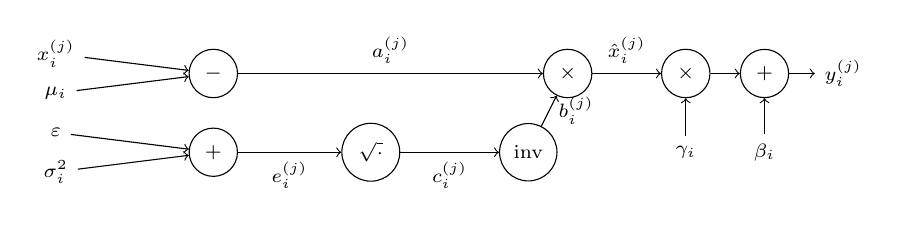
\begin{tikzpicture}[font=\scriptsize]
    \node (x) at (0, 0.25) {$x_i^{(j)}$};
    \node (mu) at (0, -0.25) {$\mu_i$};
    \node (sub) [draw, circle] at (2, 0) {$-$};

    \node (sig) at (0, -1.25) {$\sigma_i^2$};
    \node (eps) at (0, -0.75) {$\eps$};

    \node (add) [draw, circle] at (2, -1) {$+$};
    \node (sqrt) [draw, circle] at (4, -1) {$\sqrt{\cdot}$};
    \node (inv) [draw, circle] at (6, -1) {inv};
    \node (mult) [draw, circle] at (6.5, 0) {$\times$};
    \node (mult2) [draw, circle] at (8, 0) {$\times$};
    \node (add2) [draw, circle] at (9, 0) {$+$};
    \node (out) at (10, 0) {$y_i^{(j)}$};
    \node (gamma) at (8, -1) {$\gamma_i$};
    \node (beta) at (9, -1) {$\beta_i$};

    \draw[->] (x) -- (sub) node[midway, above] {};
    \draw[->] (mu) -- (sub) node[midway, below] {};

    \draw[->] (sig) -- (add) node[midway, above] {};
    \draw[->] (eps) -- (add) node[midway, above] {};
    \draw[->] (add) -- (sqrt) node[midway, below] {$e_i^{(j)}$};
    \draw[->] (sqrt) -- (inv) node[midway, below] {$c_i^{(j)}$};
    \draw[->] (sub) -- (mult) node[midway, above] {$a_i^{(j)}$};
    \draw[->] (inv) -- (mult) node[midway, right] {$b_i^{(j)}$};
    \draw[->] (mult) -- (mult2) node[midway, above] {$\hat{x}_i^{(j)}$};
    \draw[->] (mult2) -- (add2) node[midway, above] {};
    \draw[->] (gamma) -- (mult2) node[midway, below] {};
    \draw[->] (beta) -- (add2) node[midway, below] {};
    \draw[->] (add2) -- (out) node[midway, below] {};
\end{tikzpicture}
\vspace{-1em}
\end{center}
Then omitting the subscript $i$,
\newcommand{\dxhat}{\pd{\L}{\hat{x}^{(j)}}}
\newcommand{\dbeta}{\pd{\L}{\beta}}
\newcommand{\dgamma}{\pd{\L}{\gamma}}
\newcommand{\dmu}{\pd{\L}{\mu}}
\newcommand{\da}{\pd{\L}{a^{(j)}}}
\newcommand{\de}{\pd{\L}{e^{(j)}}}
\newcommand{\inv}{\frac{1}{\sqrt{\sigma^2 + \eps}}}
\newcommand{\dsig}{\pd{\L}{\sigma^2}}
\newcommand{\sumj}{\sum_{j = 1}^{m}}
\begin{align*}
    \pd{\L}{\beta} &= \sumj \pd{\L}{y^{(j)}} \\
    \pd{\L}{\gamma} &= \sumj \pd{\L}{y^{(j)}} \hat{x}^{(j)} \\
    \pd{\L}{\hat{x}^{(j)}} &= \pd{\L}{y^{(j)}} \\
    \pd{\L}{a^{(j)}} &= \inv \dxhat \\
    \pd{\L}{\mu} &= \inv \sumj \dxhat - \dsig \frac{1}{m} \sumj \frac{2(\x^{(j)} - \mu)}{m} \\
    \pd{\L}{b^{(j)}} &= \left(x^{(j)} - \mu\right) \dxhat \\
    \pd{\L}{c^{(j)}} &= -\inv \left(x^{(j)} - \mu\right) \dxhat \\
    \pd{\L}{e^{(j)}} &= -\frac{1}{2(\sigma^2 + \eps)^{\nicefrac{3}{2}}} \dxhat \\
    \dsig &= \sumj \de \\
    \dxhat &= \da + \pd{\sigma^2}{x^{(j)}} \dsig + \pd{\mu}{x^{(j)}} \dmu
\end{align*}
\end{small}
\newcommand{\wtheta}{\widetilde{\theta}}
$\wtheta = \theta + \alpha \v$. Then $\theta_{old, new} = \wtheta_{old, new} - \alpha \v_{old, new}$
Then $v_{new} = \alpha \v_{old} - \eps \grad{\theta}{\L}(\theta_{old} + \alpha \v_{old})$ so
$\pd{\L(\wtheta_{old})}{\wtheta} = \pd{\theta}{\wtheta} \pd{\L(\wtheta_{old})}{\theta} =
\pd{\L(\wtheta_{old})}{\theta}$. So
$\wtheta_{old} - \alpha \v_{new} = \theta_{old} - \alpha \v_{old} + \alpha + \v_{new}$ becomes
$\wtheta_{old} = \theta_{old} + \v_{new} + \alpha(\v_{new} - \v_{old})$, so we are done.
\newline
$\widetilde{\L}(\theta \mid \X, \y) = \L(\theta \mid \X, \y + \frac{\alpha}{2} \|\theta\|_2^2$. Then
$\grad{\theta}{\widetilde{\L}} = \grad{\theta}{\L} = \grad{\theta}{\L} + \alpha \theta$. Then
$
\theta \ot \theta - \eps \grad{\theta}{\widetilde{\L}}
\implies (1 - \eps \alpha) \theta - \eps(\grad{\theta}{\L(\theta \mid \X, \y)}
$ so we are done.
\newline
Consider $g_1, \cdots g_t$ i.i.d with mean $\mu$, varience $\sigma$. Then 
$\E(\theta_t) = \E(\theta_0) + \sum_{i = 1}^{t} v_i$ where $g_i = \mu$,
$\theta_t = \theta_{t - 1} + \v_t$ with $\E(\theta_0) = \theta_0$, and 
$\v_t = -\eps \sum_{j = 1}^{t} g_j \alpha^{t - j} = -\eps \mu \sum_{j = 1}^{t} \alpha^{t - j}$ to
get
$\E(\theta_t) = \E(\theta_0) + \sum_{i = 1}^{t} \sum_{j = 1}^{t} \alpha^{t - j}$ where $g_i = \mu$,
\newline
\bf{Mapping}
The gradient along the $\w_2$ direction is higher than the gradient along $\w_1$, direction. This is
because the contour lines along $\w_2$ directions are very close to each other which indicates a
steep curve in the $\w_2$direction. The contour lines along $w_1$ direction are further apart and
hence has slower descent. (or lower gradient)
\newline
\bf{Infinity norm}
\newline
\newcommand{\LSE}{\text{LSE}}
$\|\x\| = \max\{|x_i|\}$, $\LSE(\x) = \sum e^{x_i}$. Show
$\|\x\|_{\infty} \leq \LSE(\x) \leq \|x\|_{\infty} + \ln(n)$. Then
$n = 1 \to x \leq x \leq x + 0$. \checkmark
\newline
$n = n + 1 \to x \leq \LSE(\x) = \x + \ln(n + 1)$ so 
$e^x \leq \sum_{i = 1}^{n + 1} e^{x_i} \leq e^{x + \ln(n + 1)}$ or
\newline
$e^x \leq \sum_{i = 1}^{n} e^{x_i} + e^{x_{n + 1}} \leq (n + 1)e^{x} = ne^x + e^x$. By the inductive hypothesis, 
$\sum e^{x_i} \leq ne^x$ but since $e^{x_i} \leq e^x$, we have
$e^x \leq \sum_{i = 1}^{n} e^{x_i} + e^{x_{n + 1}} \leq (n + 1)e^{x}$, so we are done. \checkmark
\newline
To show $\|\x\|_{\infty} \leq \frac{1}{t} \LSE(t\x) \leq \|x\|_{\infty} + \frac{1}{t} \ln(n)$, set
$\x := t\x$. Then we are done.

\end{document}
